
\chapter{Appendix}
\label{chap:appendix}

\section{Further discussion about total assocaited yield per trigger particle}
\label{sec:in_depth_Y}

 A simple subtraction of $B$ from $S$ is not sufficient since the genuine correlations are distorted by the same principles discussed in sec. \ref{sec:background_distribution}. A division, however, can only be justified under two assumptions: The division would yield a distribution with a flat baseline of uncorrelated events correcting for particle pairs with one constituent outside of the detector acceptance limits $\pm\eta_m$. However, this correction is only valid if the particle densities $dN/d\eta$ of the correlated and uncorrelated particles extend beyond $\pm \eta_m$ without exceptional features. The latter is justified by studies of the pseudo rapidity presented in \cite{ALICECollaboration2012}.
Secondly, a division of $S$ and $B$ assumes that the particle densities $dN/d\eta$ of the correlated and uncorrelated particles are similar. Otherwise, the contribution from the correlated particles would be distorted differently than that of the uncorrelated ones.
While these assumptions are usually met in symmetric collisions they seem to be also suitable for many p-Pb analyzes as well \cite{ATLASCollaboration2012,Abelev2012,CMSCollaborationChatrchyan2013}.


\section{Biases in two-particle correlation functions}
\label{sec:st_shortcomings}

A collision can only contribute to \Y if it has at least one reconstructed trigger (cf. sec. \ref{sec:signal_distribution}). Thus, an event is lost to the analysis if none of its triggers were reconstructed; a scenario whose probability to occur is given by
\begin{equation}
  \label{eq:prob_one_trigger}
  P = 1 - \prod_{i}^{N}(1- \epsilon_i)
\end{equation}
where $N$ is the total number of produced trigger particles and $\epsilon_i$ is the detector efficiency for each particle $i$ given as $\epsilon(\eta_i, \varphi_i, p_{\text{T},i}, z_{\text{vtx},i})$. Figure \ref{fig:trigger_distribution} (left) shows how the distribution of the number of triggers varies between MC-truth and MC-reconstructed data. The right hand plot displays that this effect also depends on the requirement of a high \pt threshold particle: The mean number of triggers of events with such a particle is increased in comparison to the original event sample.
\begin{figure}[htbp]
  \centering
  \begin{subfigure}[b]{0.5\textwidth}
      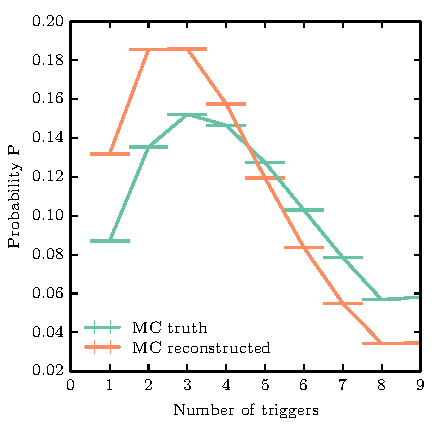
\includegraphics{figures/distribution_triggers.pdf}
  \end{subfigure}%
  \begin{subfigure}[b]{0.5\textwidth}
    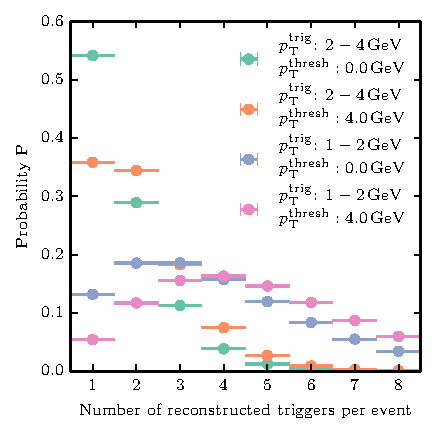
\includegraphics{figures/trigger_distribution.pdf}
  \end{subfigure}
  \caption[Investigation into trigger multiplicity effects.]{Investigation into trigger multiplicity effects. Left: Normalized distributions of the number of triggers within an event for MC-truth and MC-reconstructed data in the \pttrig interval is $1-\SI{2}{GeV/c}$. Right: Distributions for reconstructed data in different \pttrig intervals with and without a high \pt threshold.}
  \label{fig:trigger_distribution}
\end{figure}

It is well possible that an events particle density distribution, which manifests itself in the \B (eq. (\ref{eq:fancy_bg_2})) and hence \Sig, depends on the number of triggers produced in a collision. Eq. (\ref{eq:prob_one_trigger}) states that the chance of an event contributing to the analysis also depends on its number of trigger. Thus, a bias towards events with a higher number of triggers is introduces.



\section{Alternative efficiency correction by total associated yield ratios}
\label{sec:2D_correction}
The following method was developed during this thesis to correct for the observed non closure when requiring a high \pt particle in the event selection (cf. sec. \ref{sec:closure_with_thresh}) after not succeeding to fix the analysis method in this regard. This method corrects \Y with the observed non closure. This approach introduces a strong model dependence which would require further investigation. This method was thus discarded in favor of the one discussed in sec.~\ref{sec:single-value-correction}. It was included here since it is still a valid method when investigating systematic uncertainty.

The starting point of this method is the interpretation of the uncorrected ratio of $\Yrecon / \Ytruth$ as an efficiency correction $\epsilon(\deta, \dphi)$ itself. Corrected results can then be obtained by dividing $Y$  by $\epsilon(\deta, \dphi)$. However, several dependencies have to be taken into account regarding this method:

\begin{itemize}
\item As shown in fig. \ref{fig:closure_structure_w_threshold}, $\epsilon(\deta, \dphi)$ is dependent on the multiplicity class.
\item Fig. \ref{fig:closure_Y} and \ref{fig:non-closure_2-4_no_thresh} exhibit the dependence on the associated and trigger intervals.
\item Fig. \ref{fig:non-closure_2-4_no_thresh} and \ref{fig:investigate_non_closure} (left hand plot) show the scale dependence of $\epsilon(\deta, \dphi)$ on the chosen cut.
\end{itemize}

Thus, individual $\epsilon(\deta, \dphi)$ have to be computed for each of these parameters. In comparison, a single track efficiency only has to be computed once for each cut and can than be reused for all multiplicity classes, associated and trigger intervals. Hence the former method poses a much smaller degree of re-usability and generality while significantly increasing the computation requirements. 

Another issue with $\epsilon(\deta, \dphi)$ lies in the fact that it introduces unnecessary\footnote{Unnecessary in a sense that it could be overcome by having more generated MC events.} statistical uncertainties from MC data into the measurement. This shortcoming was addressed by fitting $\epsilon(\deta, \dphi)$ with a two dimensional Gaussian on the near side and an one dimensional Gaussian on the far side.

The application of this method is demonstrated for the case shown in fig. \ref{fig:closure_structure_w_threshold} (bottom right). The ratio of $\Yrecon / \Ytruth$ was fitted with the above described function. In this case the best fit yielded $\chi ^2 / NDF = 0.60$ and is displayed in fig. \ref{fig:fake_mc_closure_test} (left hand side). Dividing the initial ratio by that function yielded the results shown on the right hand side. The structure in \deta and \dphi observed in the projections of the initial ratio was successfully canceled within uncertainties in most bins. This, along with the afore stated normalized $\chi ^2$ value,  is an indicator that the chosen fit function was suitable. Albeit, it has to be noted that the statistical uncertainties at large \deta might disguise a distortion along that axis.

\begin{figure}
  \centering
  \begin{subfigure}{0.5\textwidth}
    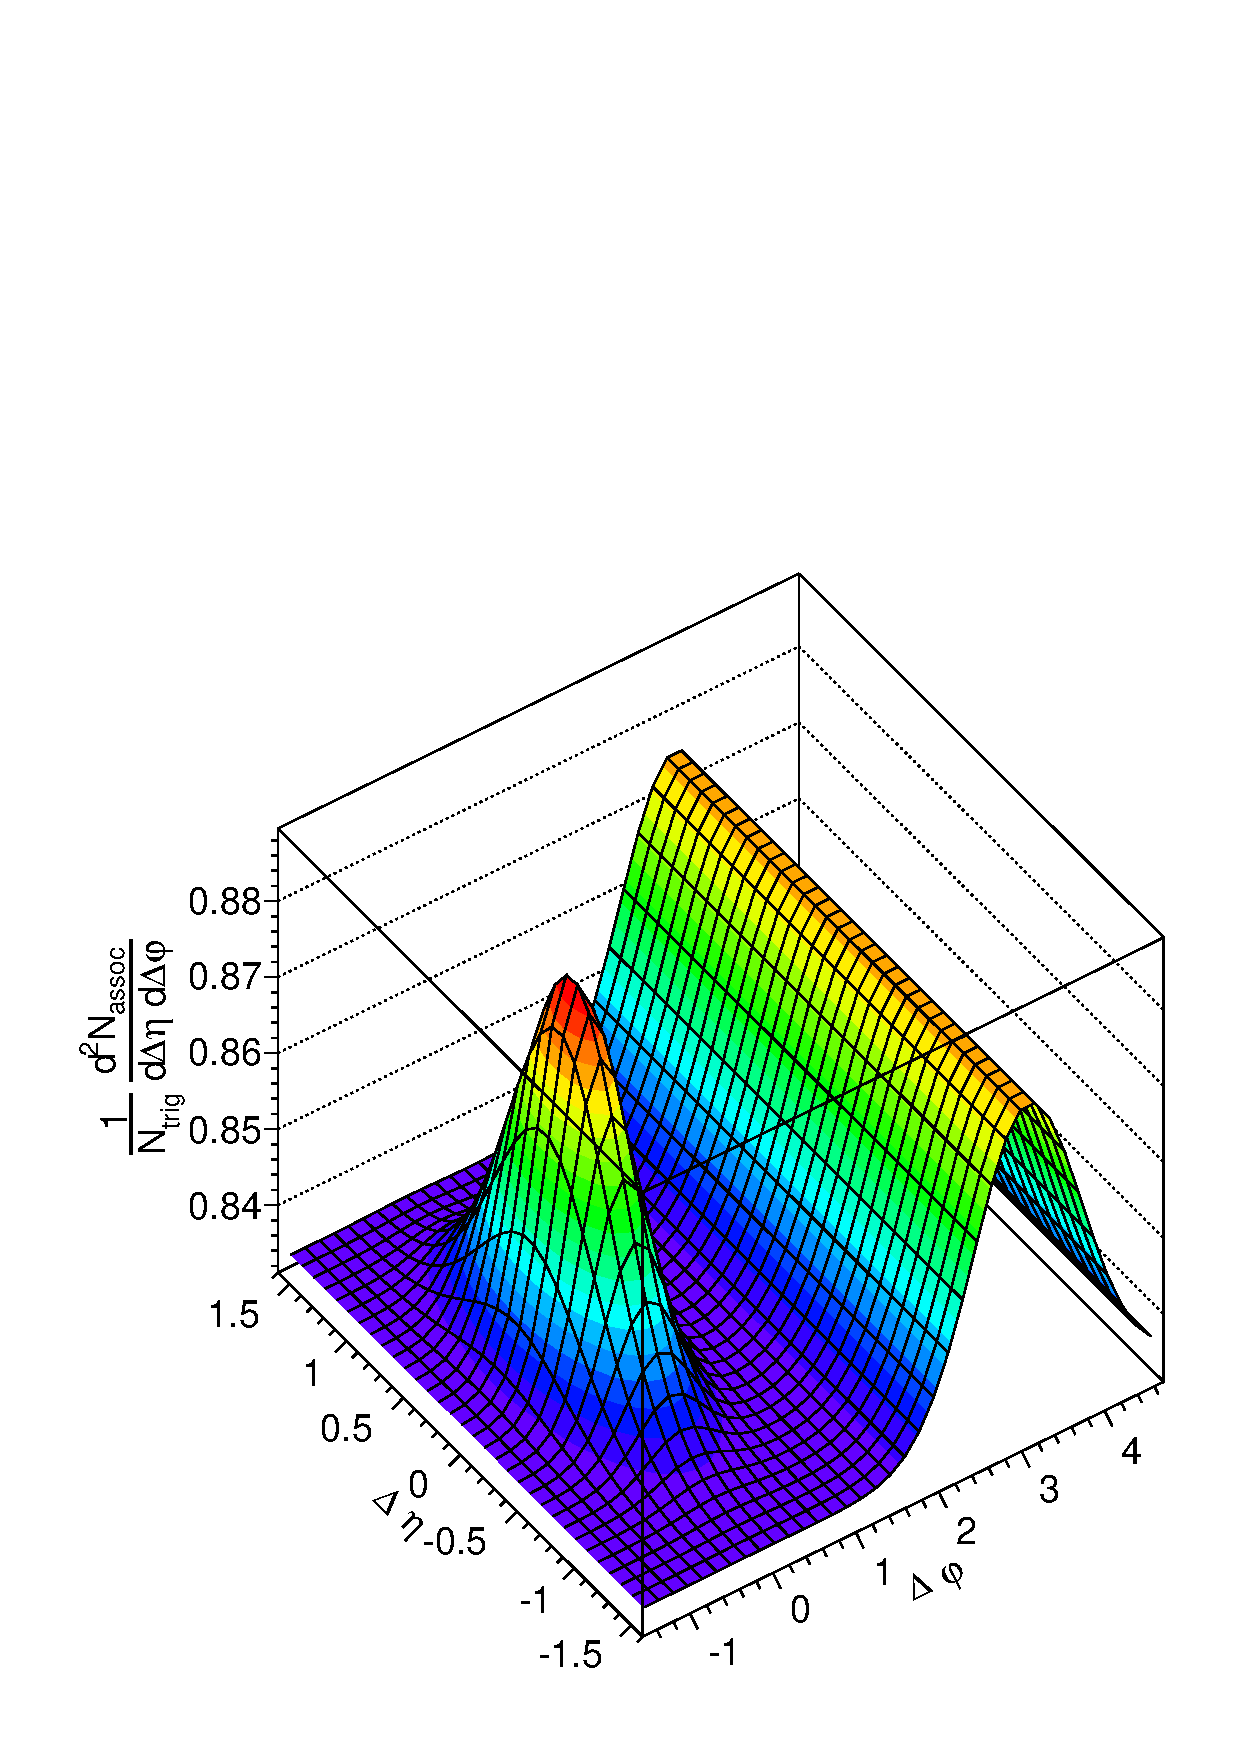
\includegraphics[width=\textwidth]{figures/fitted_function.pdf}
  \end{subfigure}%
  \begin{subfigure}{0.5\textwidth}
    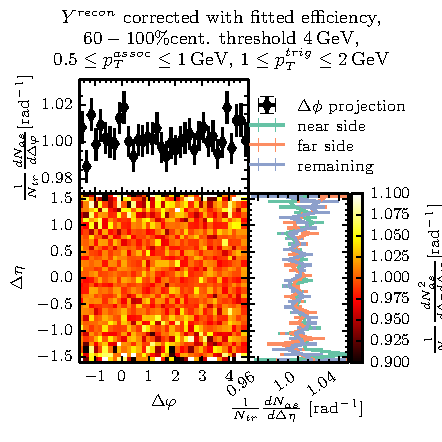
\includegraphics{figures/2d_corrected_recon.pdf}
  \end{subfigure}
  \caption[Alternative correction method based on the non-closure effects.]{Correction for non closure effects shown in fig. \ref{fig:closure_structure_w_threshold} (bottom right). Left: Non closure fitted with a two dimensional Gaussian on the \gls{near-side} and a one dimensional one on the \gls{away-side}. Right: \Yrecon corrected with the fitted function and divided by \Ytruth. }
  \label{fig:fake_mc_closure_test}
\end{figure}


%%% Local Variables: 
%%% mode: latex
%%% TeX-master: "main"
%%% End: 
